% !TeX spellcheck = en_US
% Specifica che tipo di documento vuoi creare
\documentclass[presentation,aspectratio=169]{beamer}\mode<presentation>{
% Specifica il tema da usare
\usetheme[width=2.0cm]{Hannover}
\def\swidth{2.0cm}
\setbeamertemplate{frametitle}[default][center]
\setbeamertemplate{blocks}[rounded][shadow=true]
\setbeamercolor{block body}{bg=blue!30}
%\useoutertheme{infolines}
%\setbeamertemplate{footline}[frame number]
\setbeamertemplate{sidebar left}
{
	{\usebeamerfont{title in sidebar}%
		\vskip1.5em%
		\usebeamercolor[fg]{title in sidebar}%
		\insertshorttitle[width=\swidth,center,respectlinebreaks]\par%
		\vskip1.25em%
	}%
	{%
		\usebeamercolor[fg]{author in sidebar}%
		\usebeamerfont{author in sidebar}%
		\insertshortauthor[width=\swidth,center,respectlinebreaks]\par%
		\vskip1.25em%
	}%
	\hbox to2cm{\hss\insertlogo\hss}
	\vskip1.25em%
	\insertverticalnavigation{\swidth}%
	\vfill
	\hbox to2cm{\hskip0.9cm\usebeamerfont{subsection in
			sidebar}\strut\usebeamercolor[fg]{subsection in
			sidebar}\insertframenumber\hfill}%
	\vskip3pt%
}%

}
\usecolortheme{seahorse}
% Si possono dichiarare dei pacchetti che contengono comandi aggiuntivi
\usepackage[english]{babel} % Supporta caratteri inglesi
%\usepackage[italian]{babel} % Supporta caratteri accentati italiani
\usepackage[utf8]{inputenc}

% Altri comandi aggiuntivi
\usepackage{verbatim}
%\usepackage{soul}
\usepackage{amsmath}
\usepackage{amssymb}
\usepackage{textcomp}
\usepackage[compatibility=false]{caption}
\usepackage{subcaption}
\usepackage{multicol}
\usepackage{multirow}
\usepackage{csquotes}
\usepackage[backend=bibtex,
citestyle=authoryear,
bibstyle=authoryear]{biblatex}
\usepackage{tikz}
\usepackage{gensymb}
\usepackage{setspace}
\addbibresource{literature.bib}

\defbibenvironment{bibliography}
{\list{}
	{\settowidth{\labelwidth}{\usebeamertemplate{bibliography item}}%
		\setlength{\leftmargin}{\labelwidth}%
		\setlength{\rightmargin}{\labelwidth}%
		\setlength{\labelsep}{\biblabelsep}%
		\addtolength{\leftmargin}{\labelsep}%
		\setlength{\itemsep}{\bibitemsep}%
		\setlength{\parsep}{\bibparsep}}}
{\endlist}
{\item}

%\newcommand*\oldmacro{}%
%\let\oldmacro\insertverticalnavigation%
%\renewcommand*\insertshorttitle{%
%	\oldmacro\hfill%
%	\insertframenumber}

\DeclareCiteCommand{\parencite}[\mkbibparens]
{\usebibmacro{prenote}}
{\usebibmacro{citeindex}%
	\printtext[bibhyperref]{\usebibmacro{cite}}}
{\multicitedelim}
{\usebibmacro{postnote}}

\DeclareCiteCommand{\cite}
{\usebibmacro{prenote}}
{\usebibmacro{citeindex}%
	\printtext[bibhyperref]{\usebibmacro{cite}}}
{\multicitedelim}
{\usebibmacro{postnote}}

\title[Secure and anonymous messaging]
{Secure and anonymous messaging}
%
\subtitle[Project presentation]
{Project presentation}
%
\author[Dario Pavllo]
{Dario Pavllo}
%
\institute[EPFL]
{\textsc{École polytechnique fédérale de Lausanne}\\
\rule{8cm}{.4pt}\\\smallskip
{}}
%
% Cambiate la data se volete, diversamente LaTeX mette la data odierna
\date[January 10, 2018]{January 10, 2018}

% Da qui specificate cosa deve apparire
\begin{document}
\nocite{*}

% Crea una slide per il titolo
%\frame[label=coverpage]{\titlepage}

\begingroup
\renewcommand{\insertframenumber}{}
\begin{frame}
	\addtocounter{framenumber}{0}
	\titlepage
\end{frame}
\addtocounter{framenumber}{-1}
\endgroup

\section{Introduction}
\begin{frame}{1 - Introduction}
	\textbf{Goal:} build a robust, scalable messaging system that provides end-to-end encryption, anonymity, and spam prevention.\\
	\textbf{Why?} People are putting less trust into governments; increasing demands for privacy.\\
	Short list of features:
	\begin{itemize}
		\item Public chat room and private messaging, with authentication and integrity.
		\item Anonymous identities using self-signing names.
		\item End-to-end encryption in private messages. Only end users can decrypt contents.
		\item Spam prevention through proof-of-work
	\end{itemize}
	\begin{block}{}
		\textbf{Motivation:} messaging services like Whatsapp or Telegram already implement some of these features, but they are \textbf{centralized}. We want to build our system in a decentralized setting.
	\end{block}
\end{frame}

\section{Anonymous identities}
\begin{frame}{2 - Anonymous identities}
\begin{itemize}
\item Idea borrowed from Tor hidden services (e.g. \texttt{blockchainbdgpzk.onion}) and Bitcoin wallet addresses.
\item New user generates a public/private key pair (RSA-2048).
\item Users are identified by a name derived from the public key (e.g. \texttt{alice4jfj49dkalp}). Base32 of the first 80 bits of the SHA-256 hash of the public key.
\item Easy to verify identities (names are \textbf{self-signing}).
\item No name system, no key directory, fully decentralized. Intrinsically resistant to MITM and impersonation.
\item No consensus required for registering new names.
\end{itemize}
\end{frame}

\section{Private messaging}
\begin{frame}{3 - Private messaging}
\begin{itemize}
\item \texttt{alice4jfj49dkalp} wants to send a message to \texttt{bob3fk1f94olfpoz}.
\item Alice encrypts the message with Bob's public key, and signs it using her own private key.
\item Nodes distribute the message without being able to see the content.
\item Bob decrypts the message with his private key and verifies it with Alice's public key.
\item Secure against attacks: all nodes validate signatures; public keys are verifiable.
\item Additional privacy/security: RSA-OAEP padding scheme, conflict handling.
\end{itemize}
\end{frame}

\section{Proof-of-work}
\begin{frame}{4 - Proof-of-work}
\begin{itemize}
	\item Clients must solve a crypto puzzle before sending a new message.
	\item This provides a rate-limiting mechanism against spam.
	\item A nonce is appended to the message. The SHA-256 of the message + nonce must start with N leading zeros.
	\item \textbf{Only the original sender computes the nonce!} Intermediary nodes verify it and store it along with the message.
\end{itemize}
{
	\centering
	\resizebox{1.0\textwidth}{!}{
	\begin{tabular}[c]{|l|l|l|l|l|l|l|}
		\hline
		Message ID & From & To & Content & Signature & PoW nonce\\
		\hline
		1234 & \texttt{alice4jfj49dkalp} & \texttt{bob3fk1f94olfpoz} & Encrypted binary data & 256 bytes & 16 bytes\\
		\hline	
	\end{tabular}}
	\vspace{2mm}
}\\
\end{frame}

\section{Message exchange}
\begin{frame}{5 - Message exchange}
\begin{itemize}
\item Public key sent as public message (first message)
\item Full nodes store the entire database of messages
\end{itemize}
	\begin{figure}[H]
		\centering{}
		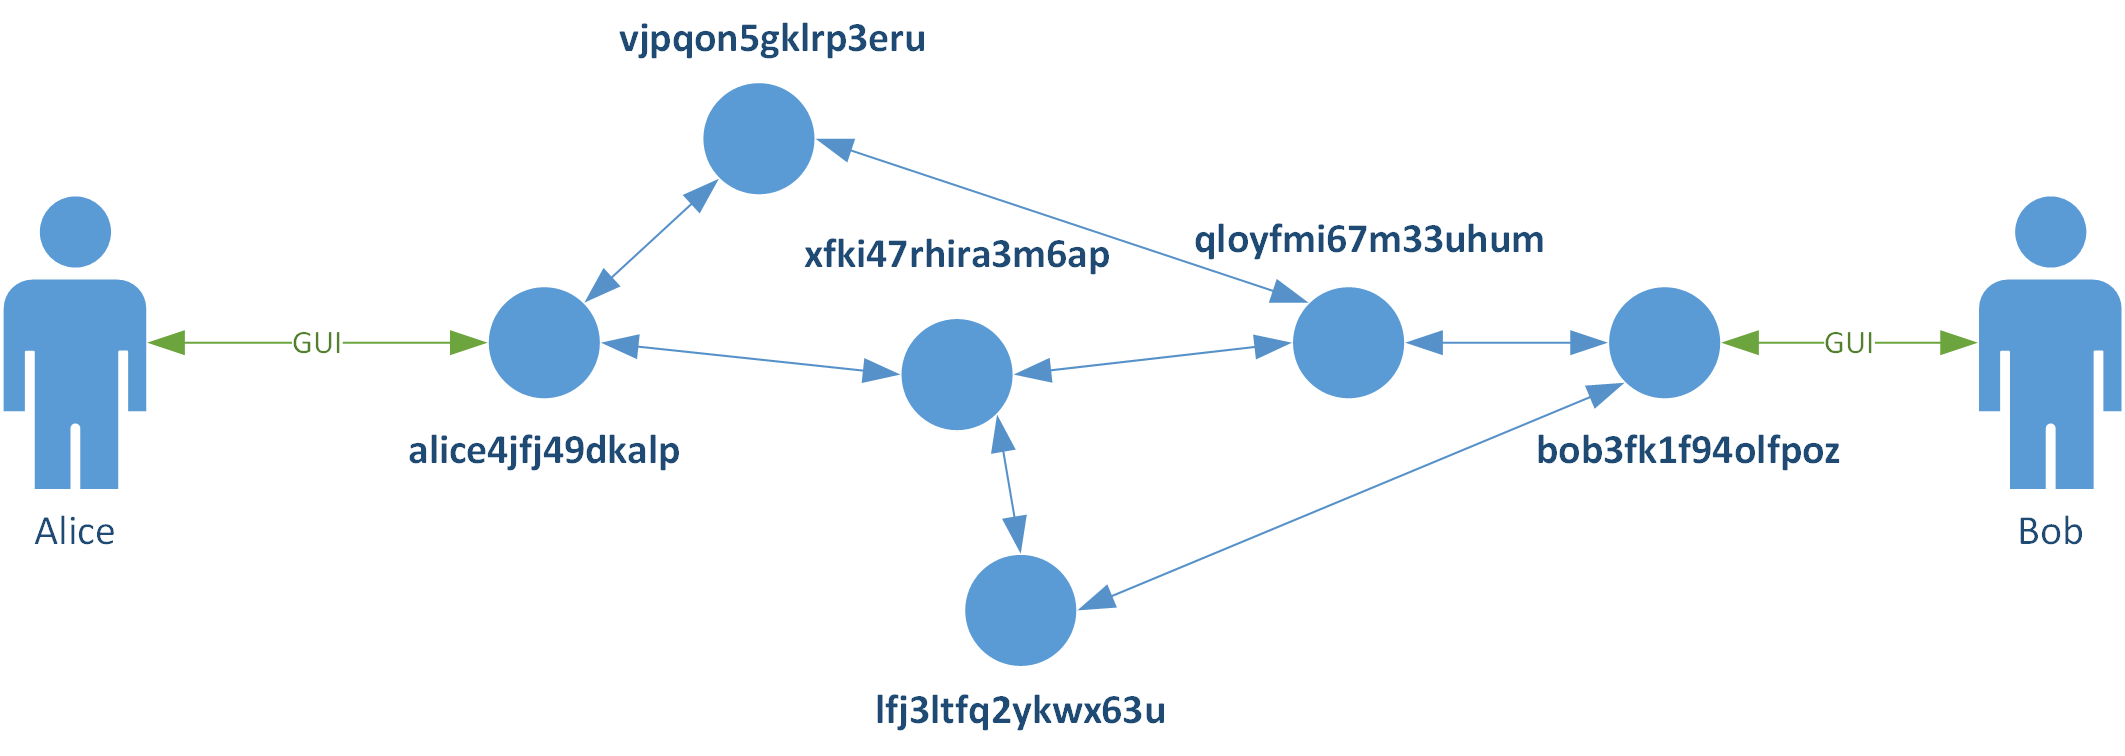
\includegraphics[width=\textwidth]{img/figure.png}
		\caption{Diagram that illustrates how users communicate.}
		\label{fig:figure}
	\end{figure}
\end{frame}




%\begin{frame}[t,allowframebreaks]
%\printbibliography
%\end{frame}

%===============================================================================
%\againframe{coverpage}
%===============================================================================
%%%%%%%%%%%%%%%%%%%%%%%%%%%%%%%%%%%%%%%%%%%%%%%%%%%%%%%%%%%%%%%%%%%%%%%%%%%%%%%%
\end{document}
%%%%%%%%%%%%%%%%%%%%%%%%%%%%%%%%%%%%%%%%%%%%%%%%%%%%%%%%%%%%%%%%%%%%%%%%%%%%%%%%